%tex
%% $Id: arbeit.tex 78 2009-07-30 19:49:33Z miracle $
% Bitte verwenden Sie pdflatex.
% Bitte beachten: es mu"s hier eine Sprachangabe gemacht werden.
% Verwenden Sie im Zweifelsfall ngerman.
\documentclass[IN,ngerman,utf8,12pt]{tumbook}
% Optionen f"ur tumbook:

%  Fakult"aten:
%   NEUTRAL -- ohne Logo und Bezeichnung
%   AR   Architektur            BV   Bauingenieur- und Vermessungswesen
%   CH   Chemie                 EI   Elektro- und Informationstechnik
%   IN   Informatik             MA   Mathematik
%   MED  Medizin                MW   Maschinenwesen
%   PH   Physik                 SE   TUM School of Education
%   SP   Sportwissenschaft      WI   Wirtschaftswissenschaften
%   WZW  Wissenschaftszentrum Weihenstephan

%   Sprachen (f"ur Silbentrennung): ngerman, english (siehe babel)
%   Schriftgr"o"sen: 9pt, 10pt, 12pt

\newcommand\todo[1]{\textcolor{red}{TODO: #1}}

\newcommand{\zB}{z.\,B.\ }
\newcommand{\ua}{u.\,a.\ }
\newcommand{\dah}{d.\,h.\ }
\newcommand{\vgl}{vgl.\ }
\newcommand{\oae}{o.\,ä.\ }
\newcommand{\vlt}{vlt.\ }
\newcommand{\bzw}{bzw.\ }
\newcommand{\ggf}{ggf.\ }
\newcommand{\va}{v.\,a.\ }
\newcommand{\Va}{V.\,a.\ }

\usepackage{epstopdf}

\makeindex

% Die klein geschriebenen \title, \author und \date sind obligatorisch.
\Seminar{ETI-Großpraktikum}
\Semester{SS 2013}
\title{Entwicklung eines Logic Analyzers in VHDL}
\Untertitel{ETI-GP 03}
\Themensteller{Georg Acher}
\TUMAdresse{Boltzmannstraße 3, 85748 Garching}
%\Autorenadresse{Anschrift und Telefonnummer des Autors}
%\Matrikelnummer{Matrikelnr. ggf. mit \, gruppiert}
%\Fachsemester{Anzahl der Fachsemester des Autors}
\Abgabetermin{10. August 2013}
\author{Sven Hertle, Markus Engel, Thomas Czok}
%\date{Ort und Datum (f\"ur ehrenw\"ortliche Erkl\"arung)}

\begin{document}
\maketitle%                  Erzeugt die Titelseite
\tableofcontents%            Erzeugt das Inhaltsverzeichnis
\clearpage

\chapter{Was ist ein Logikanalyzer?}
Mit einem Logikanalyzer kann der zeitliche Verlauf von digitalen Signalen aufgenommen werden.

Ein Logikanalyzer stellt also nur Low- und High-Pegel dar, wobei manche Geräte zusätzlich auch anzeigen können, wenn der aufgenommene Wert undefiniert ist.
Im Gegensatz zu einem Oszilloskop hat ein Logikanalyzer eine große Zahl an Kanälen, teilweise sind Geräte mit mehreren hundert Eingängen verfügbar.
Logikanalyzer werden zum Debuggen von digitalen Schaltungen benötigt.
Für diesen Zweck müssen sie mit einem großen Speicher ausgestattet sein oder sehr gute Möglichkeiten zum Triggern besitzen, da man kaum periodische Vorgänge untersuchen will.

Inzwischen werden Logikanalyzer oft durch Simulationen ersetzt.
Diese können einen Logikanalyzer aber nicht komplett ersetzen.
Auch gegenüber den Diagnoseschnittstellen, die oft in integrierten Schaltkreisen vorhanden sind, hat ein Logikanalyzer Vorteile: Dieser ist oft schneller und genauer.

\chapter{Verwendete Hardware}
\label{kap:hardware}
Der Logikanalyzer wurde mit dem FPGA-Board GOP\_XC3S200 realisiert.
Dieses ist ausgestattet mit einem Xilinx Spartan 3 XC3S200, der mit 49.152 MHz getaktet wird.
Außerdem befinden sich auf dem Board zwei Taster und acht ansteuerbare LEDs.
Diese wurden aber nicht verwendet, da noch weitere sieben Taster an das Board angeschlossen sind.
Das FPGA-Board ist mit zwei Stiftleisten direkt in einem Steckbrett angebracht.
Darüber sind die weiteren Ein- und Ausgänge sowie die Stromversorgung angeschlossen.

Die aufgezeichneten Daten können über VGA an einem Bildschirm angeschaut werden.
Für den VGA-Ausgang werden die Signale HSYNC, VSYNC sowie analoge Werte für die Farben rot, grün und blau benötigt.
Für diese analogen Werte werden jeweils zwei digitale Ausgänge über passende Widerstände zusammengeführt.
Dadurch können 64 verschiedene Farben dargestellt werden.

Der Dateneingang ist 8 Bit breit, es können also acht Kanäle aufgezeichnet werden.
Dazu befindet sich auf dem Steckbrett ein Zählbaustein, der durch einen Quarzoszillator mit 25 MHz Taktfrequenz hochgezählt wird.
Dieser dient dem Logikanalyzer als beispielhafte Signalquelle.

\begin{figure}
    \centerline{
        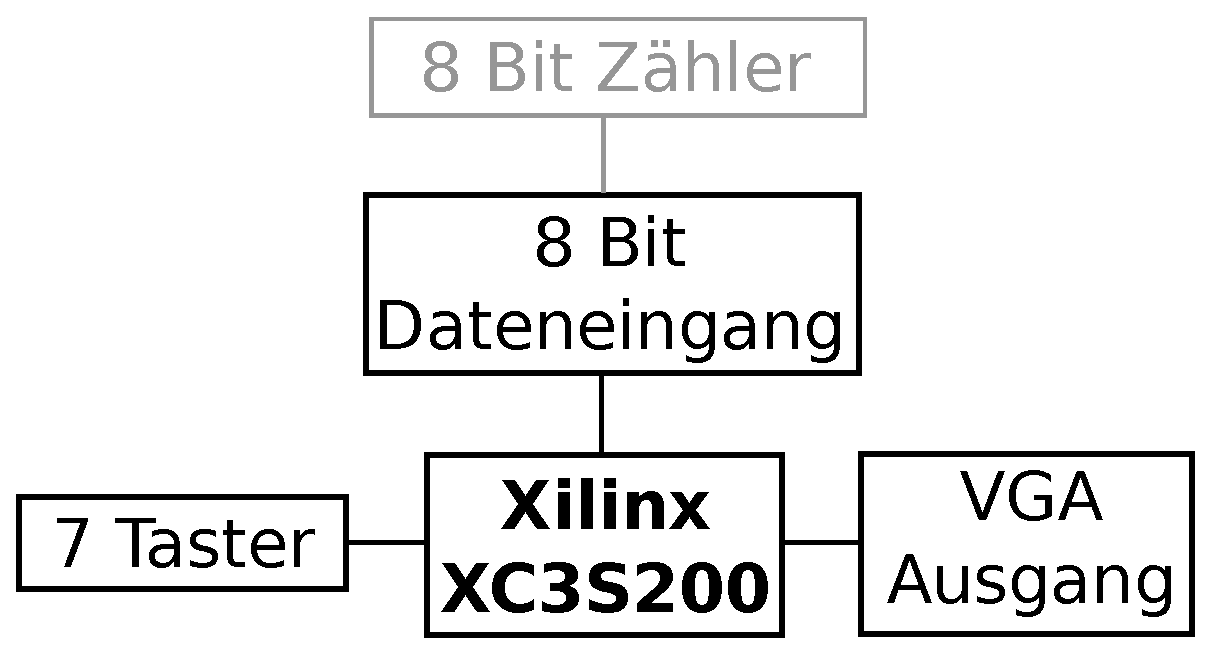
\includegraphics[width=0.5\textwidth]{img/hardware}
    }
    \caption{Schematische Darstellung der Hardware}
\end{figure}

\chapter{Spezifikation der Funktionen}

Unser Logikanalyzer kann acht Kanäle aufzeichnen.
Die Steuerung geschieht über die sieben Taster.
Die VGA-Ausgabe erzeugt ein 640x480 Pixel Bild bei 60 Hz.

Es gibt grundsätzlich zwei Aufzeichnungsarten:

\begin{description}
    \item[Continuous] Der Speicher wird als Ring verwendet, \dah die Messdaten werden ständig überschrieben.
        Sobald der Speicher voll ist, wird vorne wieder angefangen zu schreiben.
    \item[One Shot] Hier wird der Speicher einmal vollgeschrieben, danach stoppt die Aufzeichnung.
        Es passen insgesamt 24.576 Messwerte in den Speicher.
        Dieser Modus ist für die Analyse der Signale meist sinnvoller.
\end{description}

Dazu können verschiedene Samplingraten gewählt werden, \dah der Abstand zwischen zwei Aufnahmen.
Dabei sind folgende Werte möglich:

\begin{itemize}
    \item Maximum (20 ns)
    \item 1 ms
    \item 10 ms
    \item 100 ms
    \item 1 s
\end{itemize}

Nach der Aufnahme können die Daten genauer betrachtet werden.
Dazu ist Scrollen und Zoomen möglich.
Dabei wird selbstverständlich eine Zeitskala und der zeitliche Abstand (Timebase) zwischen zwei Strichen angezeigt.
Zum Überfliegen der Messdaten steht schnelles Scrollen zur Verfügung, zum Ausrichten an den Zeitmarkierungen kann dann auch langsam gescrollt werden.
Beim Zoomen entspricht 100\% einem Messwert pro Pixel.
Es sind die Zoomstufen 25\%, 50\%, 100\%, 200\% und 400\% möglich.
Die Timebase wird für jede Zoomstufe und Samplingrate korrekt angezeigt.

Der Logikanalyzer ist auch mit einfachen Triggern ausgestattet.
Pro Kanal kann als Bedingung gewählt werden, dass eine logische 1, 0, eine steigende oder fallende Flanke anliegen soll.
Wenn alle Bedingungen wahr sind, startet die Aufzeichnung.

%Aufgrund der zur Verfügung stehenden Hardware-Ressourcen mussten wir diverse Einschränkungen bei der Festlegung der gewünschten Funktionen unseres Logic Analyzers vornehmen.
%
%\section{Bildspeicher}
%Durch den geringen vorhandenen Block-RAM war es uns nicht möglich, einen kompletten Bildspeicher zu implementieren. Stattdessen sind wir darauf ausgewichen, die Bildsignale direkt aus einem Prozess heraus an den VGA-Ausgang zu senden.
%
%\section{Anzahl der aufnehmbaren Samples}
%Die Anzahl der speicherbaren Messwerte wird ebenfalls ausschließlich durch den RAM beschränkt. ...
%
%\section{Positionierung von Schriftzeichen}
%Da auch die einzelnen Zeichen in einem RAM gehalten werden müssen, haben wir keine freie Positionierung vorgesehen, sondern uns darauf beschränkt, den Bildschirm in 8x8 Pixel große Quadrate (Größe eines Zeichens) zu unterteilen und jedem Quadrat ein Zeichen zuweisen zu können.
%
%\section{Maximale Samplingrate}
%Die maximale einstellbare Samplingrate hängt vom zur Verfügung stehenden Takt ab. Dieser beträgt 49,xy MHz; das entspricht der höchsten Samplingrate.

\chapter{Bedienungsanleitung für Anwender}

Der Logikanalyzer lässt sich über den vorhandenen VGA-Anschluss an einen handelsüblichen Monitor anschließen.

\begin{figure}
    \centerline{
        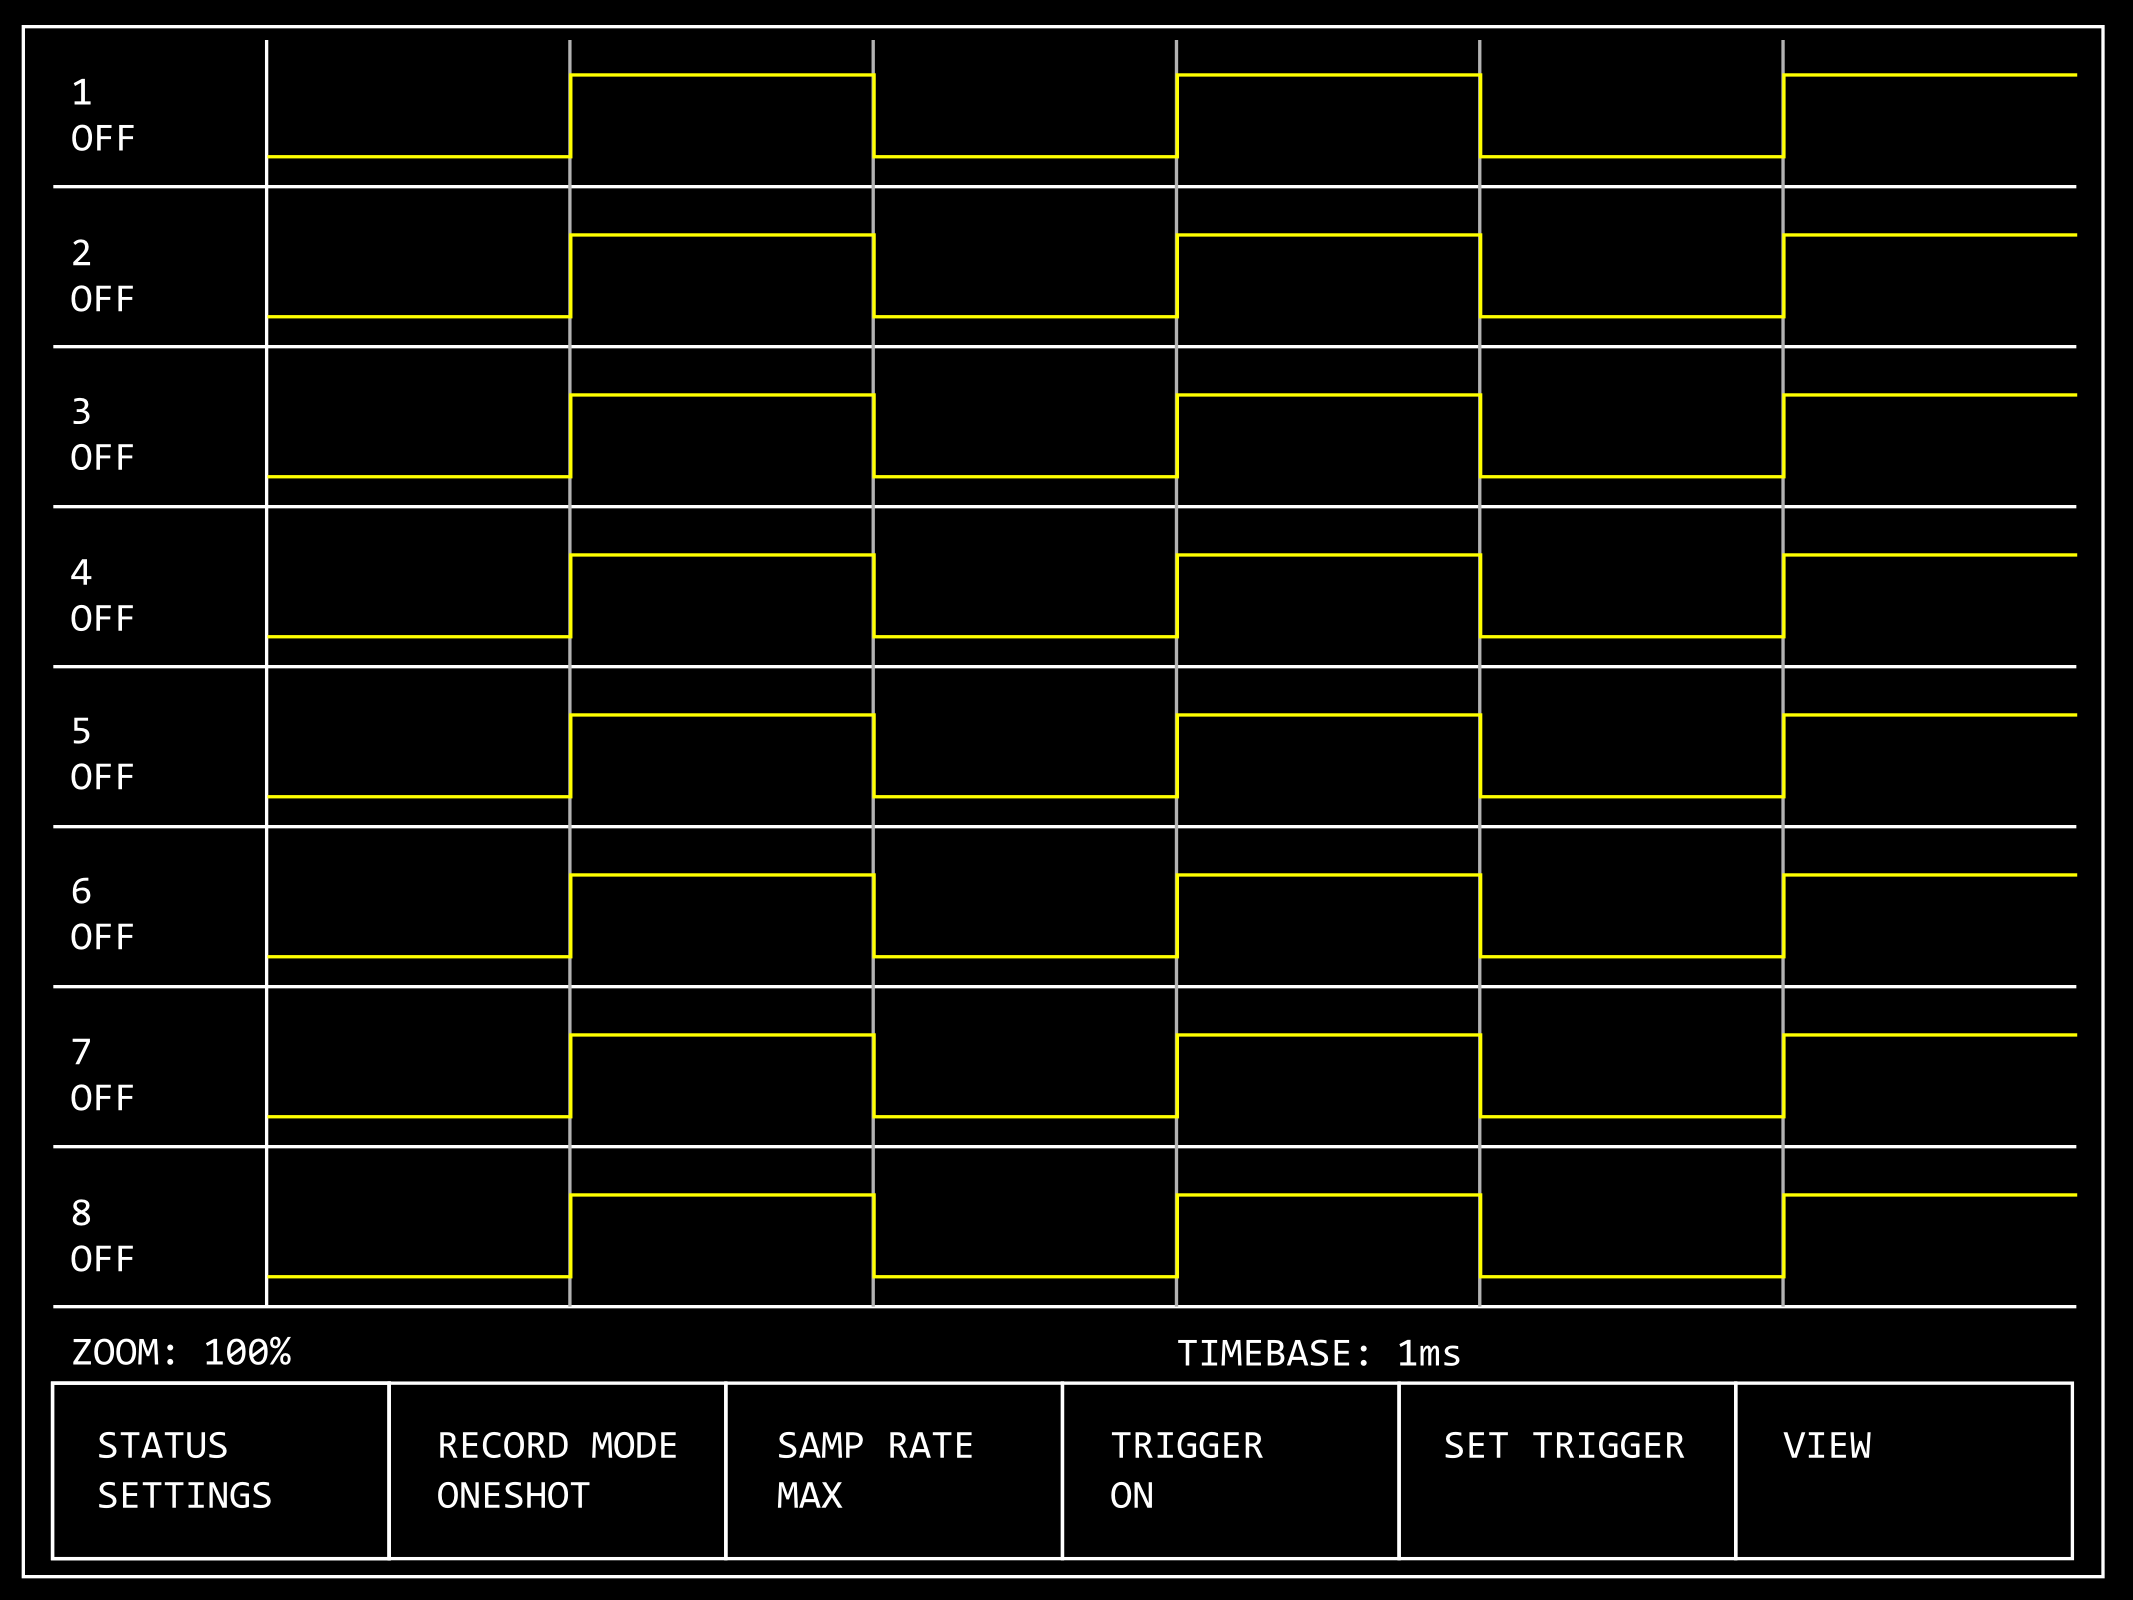
\includegraphics[width=0.75\textwidth]{img/bildschirm}
    }
    \label{abb:bildschirm}
    \caption{Bildschirmansicht des Logikanalyzers}
\end{figure}

\section{Beschreibung des Benutzerinterfaces}

Im oberen Teil der Anzeige befindet sich die Darstellung der einzelnen Kanäle, links stehen die Kanalnummer und eventuell eingestellte Trigger.
Unter der Anzeige des aktuell gewählten Zoomfaktors und der Timebase (der vergangenen Zeit zwischen zwei aufeinanderfolgenden senkrechten Strichen) liegt die Menüzeile.

Nach dem Einschalten befindet sich der Logikanalyzer zunächst im Zustand ``Settings'', in dem die Einstellungen am Aufnahmemodus, der Samplingrate und den Triggern vorgenommen werden können.

\section{Steuerung des Menüs}

Die Bedienung erfolgt über die acht zur Verfügung stehenden Taster.
\todo{Bild?}
Der momentan aktive Menüpunkt wird durch die Pfeiltasten nach links und rechts gewählt und durch einen roten Rahmen markiert. Mit den Pfeiltasten hoch und runter kann die Einstellung des aktiven Menüpunkts verändert werden.

\section{Setzen von Triggern}

Werden Trigger im Menü aktiviert, besteht die Möglichkeit, über den Menüpunkt ``Set Trigger'' in das Trigger-Untermenü zu wechseln. Dieses befindet sich am linken Rand jeweils unterhalb der Kanalnummern. Der momentan aktive Kanal wird durch einen Pfeil gekennzeichnet und kann mit den Pfeiltasten gewechselt werden. Durch die Pfeiltasten nach links und rechts kann der Trigger eingestellt werden.

Wird nach dem Setzen der Einstellungen das Menü verlassen und die Aufnahme gestartet, so beginnt diese tatsächlich erst, wenn das momentan anliegende Signal alle Bedingungen erfüllt, die durch die Trigger vorgegeben wurden.

\section{Ansicht der Messwerte}
Nachdem die Aufnahme von selbst gestoppt hat (Oneshot) oder vom Benutzer durch den Stop-Button unterbrochen wurde (Continuous), besteht die Möglichkeit im ``View''-Modus mit dem Pfeiltasten nach links und rechts zu scrollen und den Zoomfaktor zu verändern.

\chapter{Dokumentation für Entwickler}

Der Logikanalyzer wurde mit VHDL implementiert.
Dazu wurde die Software Xilinx ISE WebPACK verwendet.

\section{Komponenten}

Der Logikanalyzer ist in verschiedene Komponenten unterteilt.
Diese werden in Abb. \ref{abb:komp} dargestellt.

\begin{figure}
    \centerline{
        \includegraphics[width=0.5\textwidth]{img/komponenten}
    }
    \label{abb:komp}
    \caption{Unterteilung des Logikanalyzers in Komponenten}
\end{figure}

\subsection{Logikanalyzer}
Die Komponente ``Logikanalyzer'' übernimmt die Steuerung aller anderen Komponenten.
Sie beinhaltet alle Signale, die den Status der Logikanalyzers speichern.
Die zur Steuerung verwendeten Taster werden hier ausgewertet.
Die Signale werden dann entsprechend verändert, sodass die vom Benutzer gewünschte Aktion ausgeführt wird.

\begin{figure}[H]
    \centerline{
        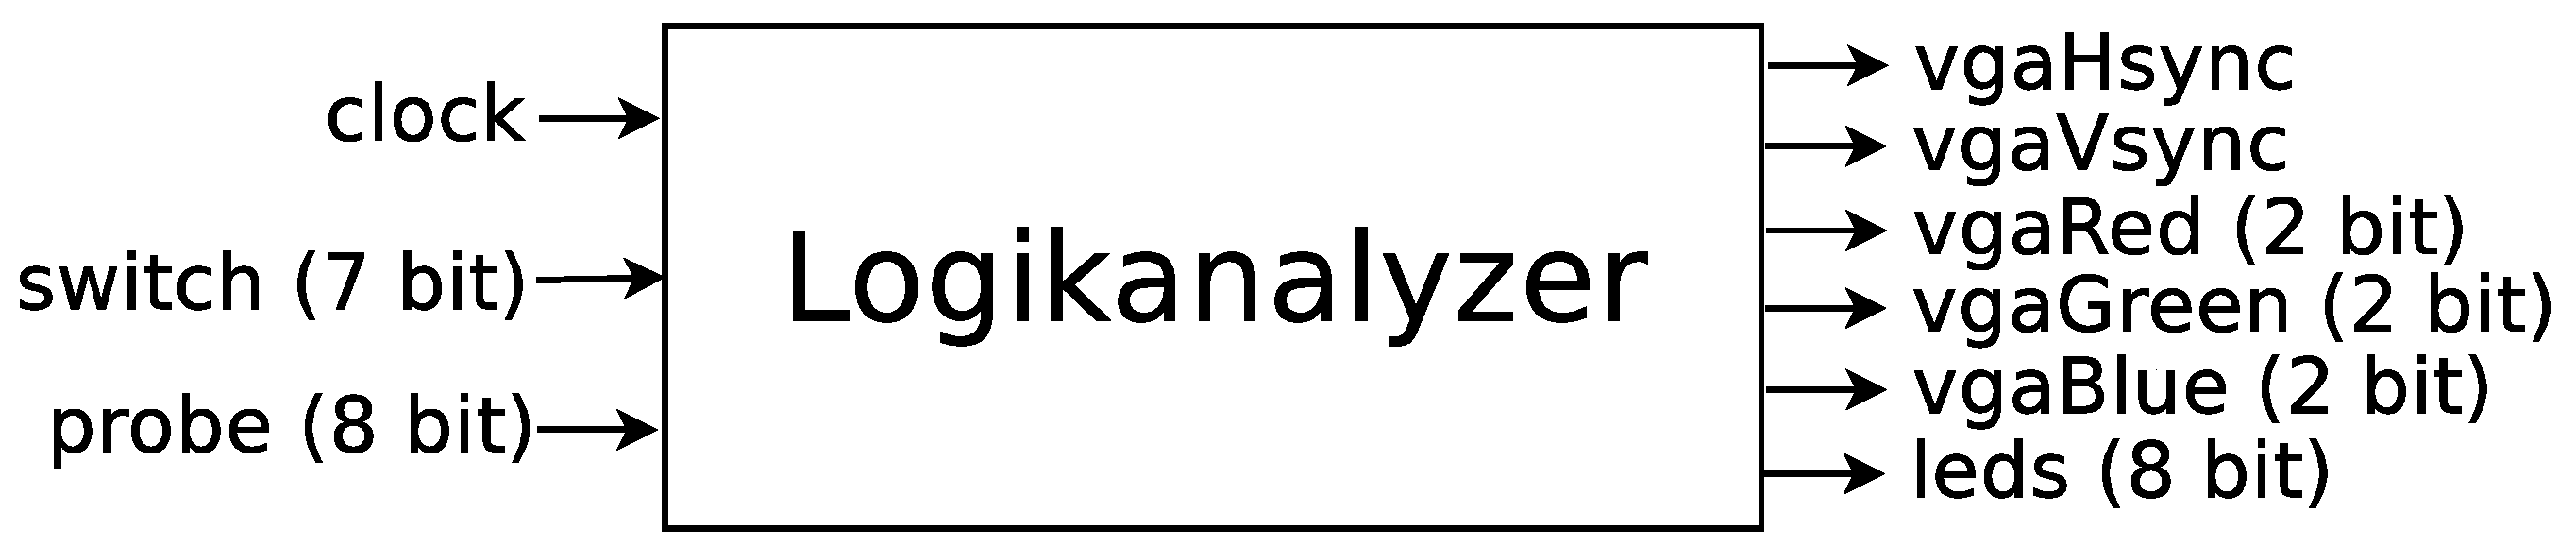
\includegraphics[width=0.75\textwidth]{img/logikanalyzer}
    }
    \label{abb:logikanalyzer}
    \caption{Ein- und Ausgänge der Komponente Logikanalyzer}
\end{figure}

Die Komponente Logikanalyzer hat diese Ein- und Ausgänge (\vgl Abb. \ref{abb:logikanalyzer}):
\begin{description}
    \item[clock] Takt des Bausteins (\texttt{std\_logic})
    \item[switch] 7 Bit breiter Eingang der externen Taster (\texttt{std\_logic\_vector(1 to 7)})
    \item[probe] 8 Bit breiter Eingang für die Messwerte (\texttt{std\_logic\_vector(7 downto 0)})
    \item[vgaHsync] HSync-Ausgang für VGA-Signal (\texttt{std\_logic})
    \item[vgaVsync] VSync-Ausgang für VGA-Signal (\texttt{std\_logic})
    \item[vgaRed] Ausgang für rote Farbkomponente des VGA-Signals (\texttt{std\_logic\_vector(1 downto 0)}, \vgl Kapitel \ref{kap:hardware})
    \item[vgaGreen] Ausgang für grüne Farbkomponente des VGA-Signals (\texttt{std\_logic\_vector(1 downto 0)})
    \item[vgaBlue] Ausgang für blaue Farbkomponente des VGA-Signals (\texttt{std\_logic\_vector(1 downto 0)})
    \item[leds] 8 Bit breiter Ausgang für LEDs (wird nur auf 0 gesetzt, \texttt{std\_logic\_vector(7 downto 0)})
\end{description}

\subsection{RAM}

Zum Speichern der Messwerte wird ein Dualport Block RAM verwendet.
Dieser hat den Vorteil, dass gleichzeitig Daten gelesen und geschrieben werden können.
Dies ist nötig, da gleichzeitig Messwerte aufgenommen und Daten auf dem Bildschirm angezeigt werden müssen.
Der RAM wurde mit dem Core Generator aus Xilinx ISE generiert.
Für Änderungen ist daher mindestens Xilinx ISE Version 14.6 nötig.

\subsection{Sampler}
\label{kap:sampler}

Der Sampler hat die Aufgabe, die Messwerte im RAM zu speichern.
Dabei muss die gewählte Samplingrate sowie der Aufnahmemodus beachtet werden.
Außerdem müssen die aktuell an den Eingängen anliegenden Messwerte an den Sampler weitergegeben werden.
Dieser braucht die aktuellen Daten, um zu entscheiden, ob die Aufnahme gestartet werden soll.

\begin{figure}[H]
    \centerline{
        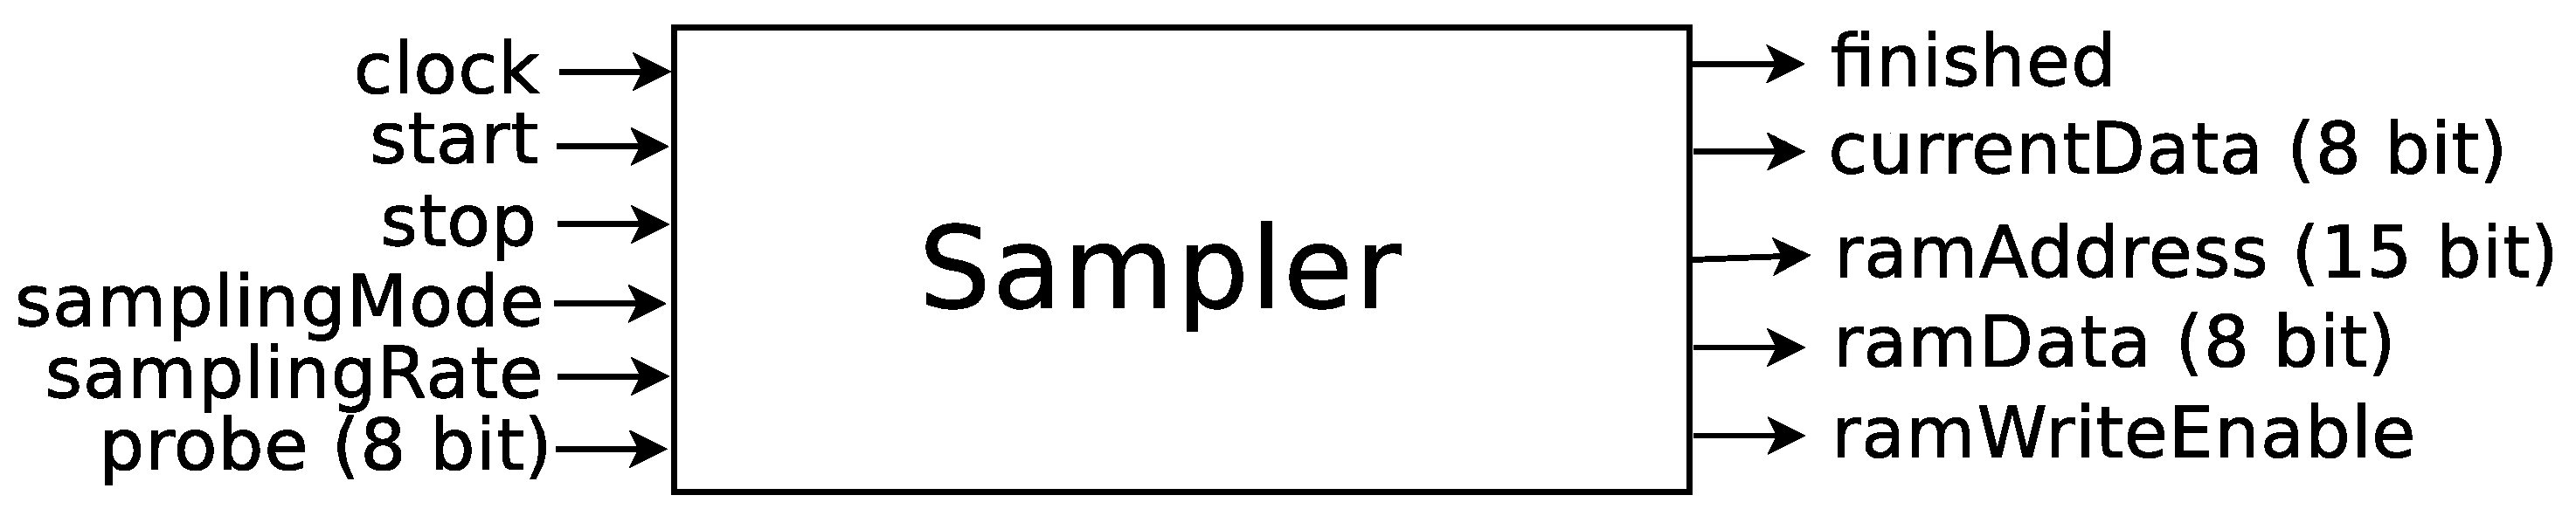
\includegraphics[width=0.75\textwidth]{img/sampler}
    }
    \label{abb:sampler}
    \caption{Ein- und Ausgänge der Komponente Sampler}
\end{figure}

Die Komponente Sampler hat diese Ein- und Ausgänge (\vgl Abb. \ref{abb:sampler}):
\begin{description}
    \item[clock] Takt des Bausteins (\texttt{std\_logic})
    \item[start] Aufnahme wird gestartet, wenn eine 1 anliegt. Diese darf nur einen Takt lang anliegen, sonst beginnt die Aufnahme wieder von vorne (\texttt{std\_logic})
    \item[stop] Stoppen der Aufnahme. Dies ist im Oneshot-Modus nicht nötig, da die Aufnahme automatisch stoppt (\texttt{std\_logic})
    \item[samplingMode] Zu verwendender Sampling Modus (\texttt{SamplingMode}, \vgl \ref{kap:samplingmode})
    \item[samplingRate] Zu verwendende Samplingrate (\texttt{SamplingRate}, \vgl \ref{kap:samplingrate})
    \item[probe] 8 Bit breiter Eingang für die Messwerte (\texttt{std\_logic\_vector(7 downto 0)})
    \item[finished] 1, wenn der Sampler mit der Aufzeichnung fertig ist. \Va für Continuous Modus wichtig (\texttt{std\_logic})
    \item[currentData] Aktuelle Messwerte am Eingang unter Beachtung der Sampling Rate und des Modus (\texttt{std\_logic\_vector(7 downto 0)})
    \item[ramAddress] Adresse für schreibenden RAM-Zugriff (\texttt{std\_logic\_vector(14 downto 0)})
    \item[ramData] Daten, die in den RAM geschrieben werden sollen (\texttt{std\_logic\_vector(7 downto 0)})
    \item[ramWriteEnable] 1, wenn im nächsten Takt in der RAM geschrieben werden soll (\texttt{std\_logic\_vector(0 downto 0)} \todo{WTF?})
\end{description}

\subsection{Trigger}

Der Trigger entscheidet, ob die Aufnahme gestartet werden soll.
Grundlage dafür sind die Einstellungen des Benutzers und die aktuellen Messwerte.

\begin{figure}[H]
    \centerline{
        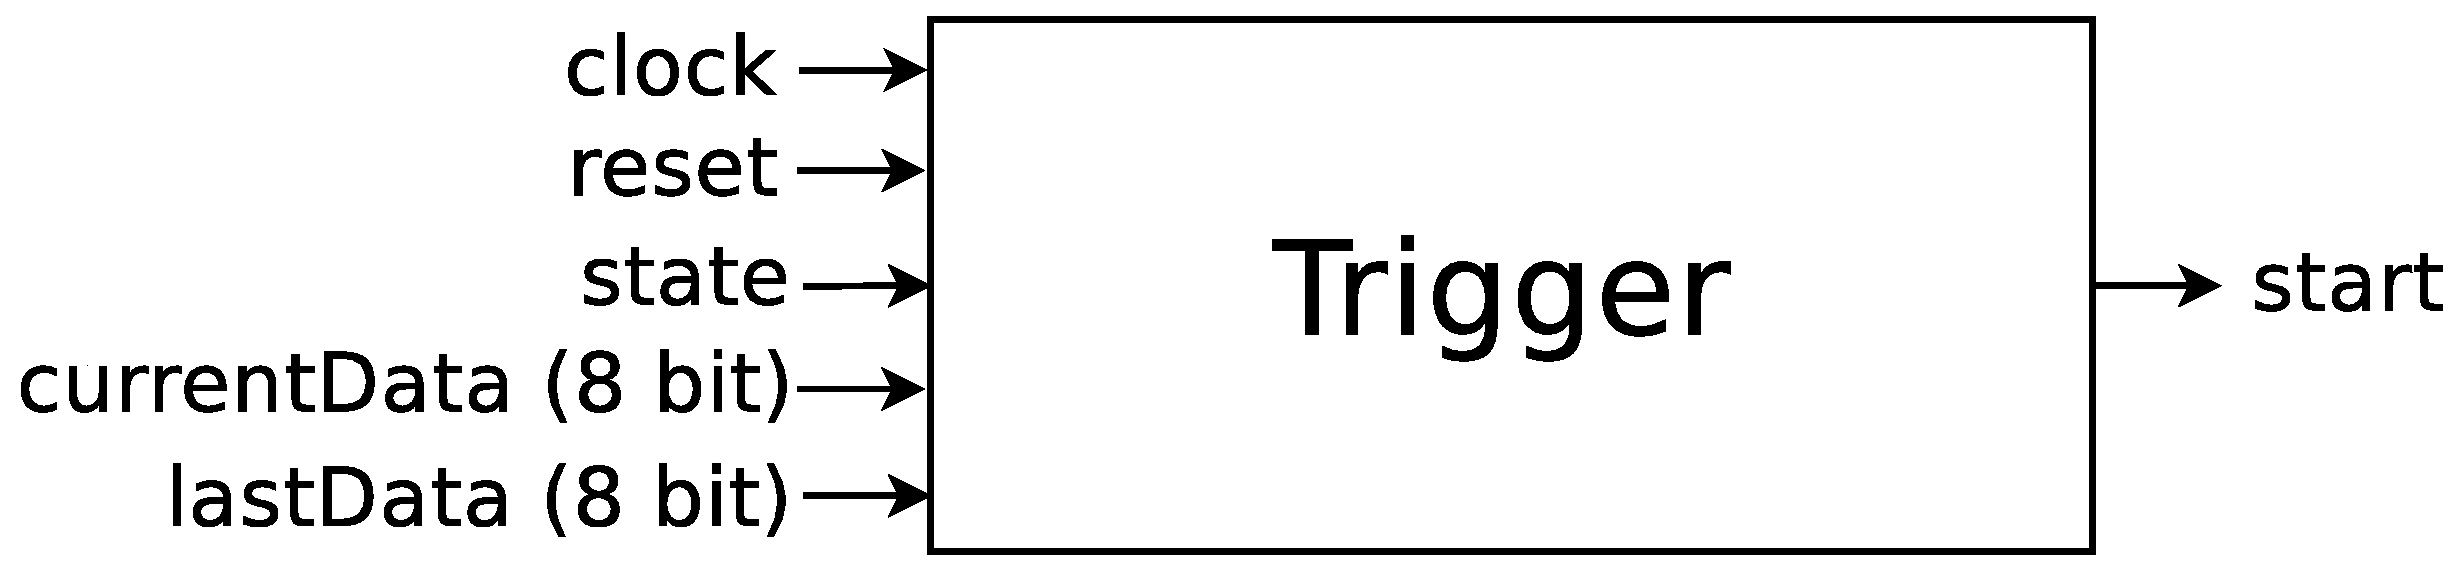
\includegraphics[width=0.75\textwidth]{img/trigger}
    }
    \label{abb:trigger}
    \caption{Ein- und Ausgänge der Komponente Trigger}
\end{figure}

Die Komponente Trigger hat diese Ein- und Ausgänge (\vgl Abb. \ref{abb:trigger}):

\begin{description}
    \item[clock] Takt des Bausteins (\texttt{std\_logic})
    \item[reset] Ausgang \texttt{start} auf 0 zurücksetzen (\texttt{std\_logic})
    \item[state] Einstellungen der Trigger für alle Kanäle (\texttt{AllTriggers}, \vgl o{ref})
    \item[currentData] Aktuelle Messwerte, die aufgenommen werden würden (\texttt{std\_logic\_vector(7 downto 0)})
    \item[lastData] Vorherige Messwerte für Flankenerkennung (\texttt{std\_logic\_vector(7 downto 0)})
    \item[start] Ausgang, der 1 ist, wenn die Trigger auslösen (\texttt{std\_logic})
\end{description}

\subsection{VGA}

Die Komponente VGA erzeugt ein VGA-Signal mit 640x480 Pixeln und 60 Hz.
Diese Größe und Frequenz wurde gewählt, da der Pixeltakt dann bei 25 MHz liegt, was grob dem halbem Takt des Bausteins (49.152 MHz) entspricht.
Die Abweichung ist klein genug, sodass sie keine Rolle spielt.

\begin{figure}[H]
    \centerline{
        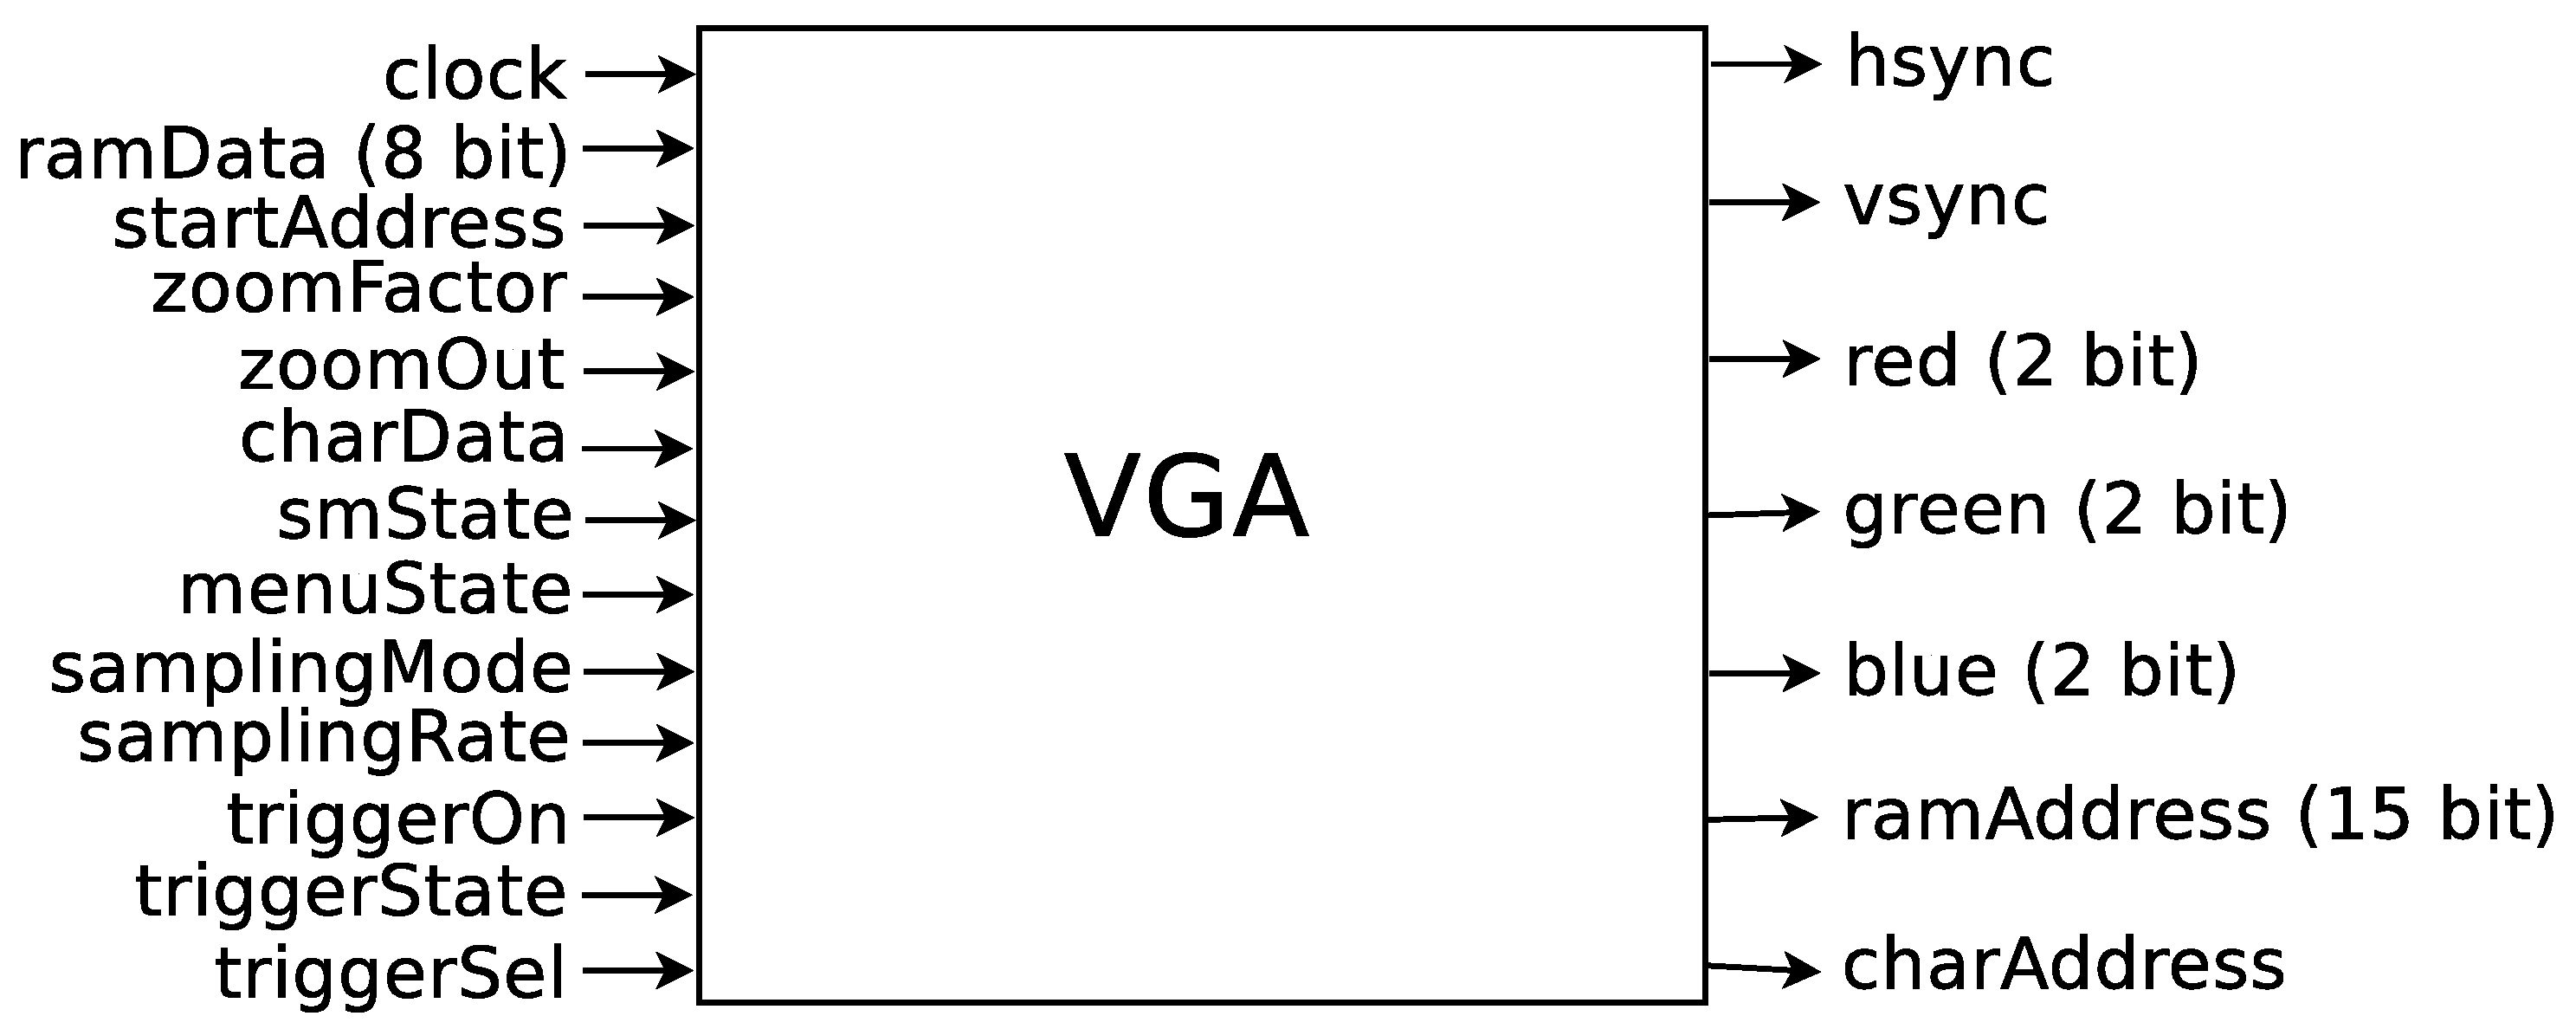
\includegraphics[width=0.75\textwidth]{img/vga}
    }
    \label{abb:vga}
    \caption{Ein- und Ausgänge der Komponente VGA}
\end{figure}

Diese Komponente bekommt als Eingabe alle Informationen über das darzustellende Bild, \vgl die Eingänge des Bausteins.

Dementsprechend wird die Ausgabe dann gezeichnet.
Da nicht genug Speicher für einen Bildspeicher verfügbar ist, wird in jedem Takt entschieden, welche Farbe der aktuelle Pixel hat.
Dazu muss man für jeden Pixel, an den etwas gezeichnet werden soll, abfragen, ob dieser aktuell gezeichnet wird.
Wenn dies der Fall ist, muss die passende Farbe auf die VGA Ausgänge gelegt werden.
Es wurden Prozeduren geschrieben, die das Zeichnen von Linien, Rechtecken und Texten übernehmen:

\begin{description}
    \item[setPixel(p: Point, c: Color)] setzt einen einzelnen Pixel
    \item[drawChar(p: Point, char : character)] zeichnet einen Buchstaben.
        Die Position muss zwischen \texttt{(0,0)} und \texttt{(79, 59)} liegen (siehe unten).
    \item[drawString(p: Point, str: string)] zeichnet einen String.
    \item[drawLine(fromP: Point, toP: Point, c:Color)] zeichnet eine Linie.
    \item[drawRectangle(upperLeft: Point, lowerRight: Point, c: Color)] Zeichnet ein Rechteck.
\end{description}

Hier wurden die Datentypen \texttt{Point} und \texttt{Color} verwendet.
\texttt{Point} ist ein Tupel aus x und y-Koordinate.
\texttt{Color} ist ein Tupel aus Rot, Grün und Blau-Wert, wobei jeder einzelne Wert 2 Bit hat.
Einige Farben wurden als Konstanten definiert, \zB \texttt{ColorBlack}.
Die vollständige Liste findet man im Quellcode.

Damit das Zeichnen der Texte nicht zu aufwändig wird, wird dafür ein Bildspeicher verwendet:
Die einzelnen Zeichen sind 8x8 Pixel groß und können nur in einem Raster mit 8 Pixel Abstand angeordnet werden.
So können insgesamt 80x60 Zeichen dargestellt werden.
Diese werden in einem Array gespeichert, was einem Bildspeicher entspricht.
Da hier aber nur die ASCII-Werte der Zeichen gespeichert werden, verbraucht dies nicht zu viel Speicherplatz.
Man muss darauf achten, dass alle Strings gleich lang sind, wenn man an eine Stelle abwechselnd unterschiedliche Texte schreiben will.
Die Prozedur \texttt{drawString} schreibt den Text in den Bildspeicher.
Wenn dieser zu kurz ist, bleibt noch das Ende der vorherigen Textes übrig.
Hier muss man also noch mit Leerzeichen auffüllen.

Beim Zeichnen der aufgezeichneten Signale werden noch steigende und fallende Flanken ergänzt.
Dabei wird einfach bei einem Wechsel des Signals eine senkrechte Linie dazu gezeichnet.

Die Komponente VGA hat diese Ein- und Ausgänge (\vgl Abb. \ref{abb:vga}):
\begin{description}
    \item[clock] Takt des Bausteins (\texttt{std\_logic})
    \item[ramAddress] Ausgang für Speicheradresse. Die Daten an dieser Adresse liegen im nächsten Takt an \texttt{ramData} an (\texttt{std\_logic\_vector(14 downto 0)})
    \item[ramData] Eingang für Daten aus dem Speicher (\texttt{std\_logic\_vector(7 downto 0)})
    \item[startAddress] Adresse des ersten darzustellenden Wertes im Speicher (\texttt{std\_logic\_vector(14 downto 0)})
    \item[zoomFactor] Eingang für Zoomfaktor: 1, 2 oder 4 für 100\%, 200\% oder 400\% (\texttt{integer})
    \item[zoomOut] Eingang, der anzeigt, ob hinein oder herausgezoomt wird: 1 bedeutet herauszoomen, 0 hineinzoomen.
        Bei Zoomfaktor 1 ist dieser Wert egal (\texttt{boolean})
    \item[charAddress] Ausgang zur Ansteuerung der TextROMs (\texttt{character})
    \item[charData] Eingang von TextROM (\texttt{Letter}, \vgl \ref{kap:letter})
    \item[smState] Eingang für Status der Logikanalyzers (\texttt{State}, \vgl \ref{kap:state})
    \item[menuState] Eingang für Status des Menüs (\texttt{Menu}, \vgl \ref{kap:menu})
    \item[samplingMode] Eingang für verwendeten Sampling Modus (\texttt{SamplingMode}, \vgl \ref{kap:samplingmode})
    \item[samplingRate] Eingang für verwendete Sampling Rate (\texttt{SamplingRate}, \vgl \ref{kap:samplingrate})
    \item[triggerOn] Eingang, der 1 ist, wenn die Trigger aktiviert sind (\texttt{boolean})
    \item[triggerState] Eingang für Einstellungen der Trigger (\texttt{AllTriggers}, \vgl \ref{kap:alltriggers})
    \item[triggerSel] Eingang für im Triggermenu gewählten Kanal (0-7). 8 bedeutet, dass das Hauptmenü ausgewählt ist. (\texttt{integer range 0 to 8})
    \item[hsync] HSync-Ausgang für VGA-Signal (\texttt{std\_logic})
    \item[vsync] VSync-Ausgang für VGA-Signal (\texttt{std\_logic})
    \item[red] Ausgang für rote Farbkomponente des VGA-Signals (\texttt{std\_logic\_vector(1 downto 0)}, \vgl Kapitel \ref{kap:hardware})
    \item[green] Ausgang für grüne Farbkomponente des VGA-Signals (\texttt{std\_logic\_vector(1 downto 0)})
    \item[blue] Ausgang für blaue Farbkomponente des VGA-Signals (\texttt{std\_logic\_vector(1 downto 0)})
\end{description}

\subsection{TextROM}

Der TextROM ist nur ein Speicher für die Schriftzeichen.
Dabei wird für einen ASCII-Wert das Zeichen als 8x8 Pixel-Grafik gespeichert.
Die Tabelle enthält aktuell nur Großbuchstaben, Zahlen und einige Sonderzeichen, um Platz zu sparen.
Die Schriftzeichen wurden aus dem Linux Kernel übernommen.

\begin{figure}[H]
    \centerline{
        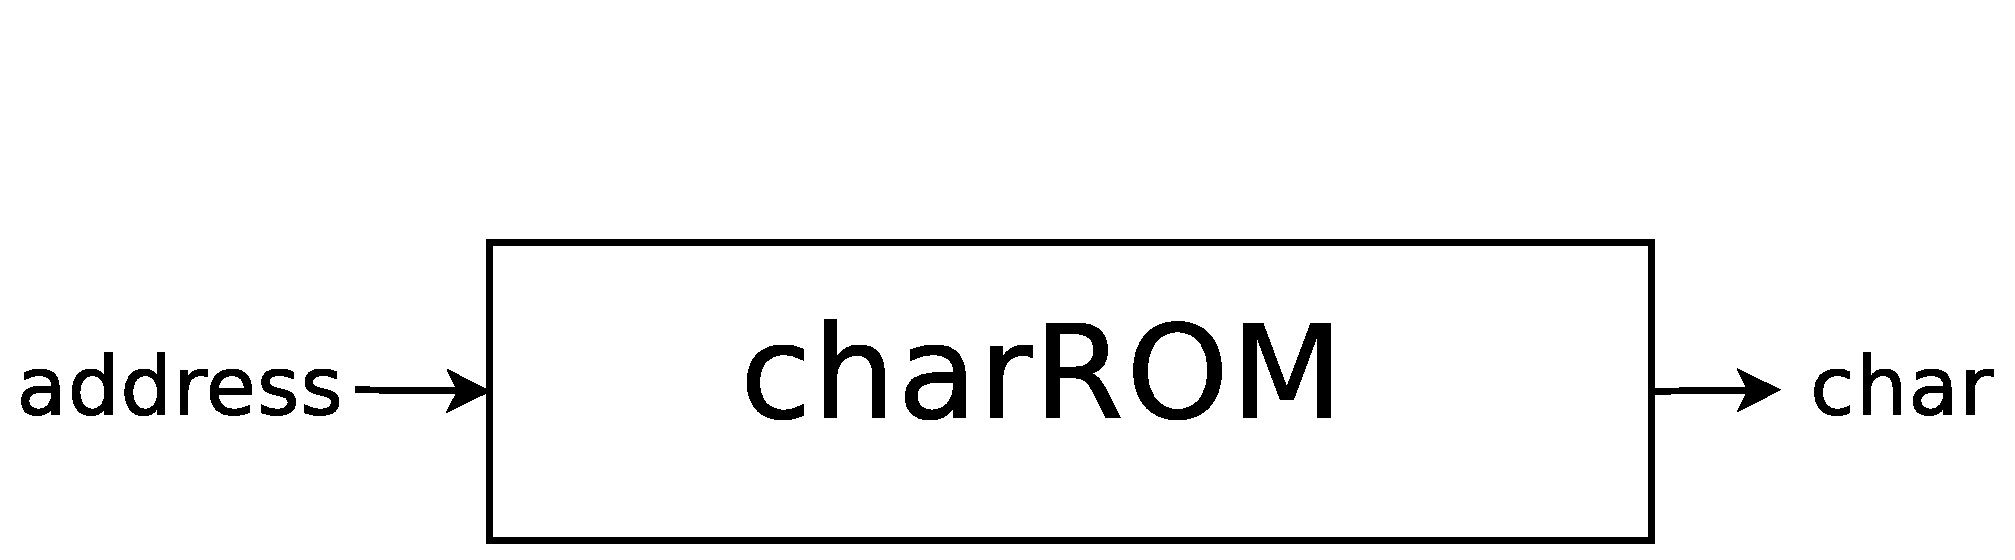
\includegraphics[width=0.5\textwidth]{img/textROM}
    }
    \label{abb:textrom}
    \caption{Ein- und Ausgänge der Komponente TextROM}
\end{figure}

Die Komponente TextROM hat diese Ein- und Ausgänge (\vgl Abb. \ref{abb:textrom}):
\begin{description}
    \item[address] Eingang mit ASCII-Zeichen (\texttt{character})
    \item[char] Ausgang mit 8x8 Pixel-Schriftzeichen (\texttt{Letter}, \vgl \ref{kap:letter})
\end{description}

\section{Eigene Datentypen}
Als Datentypen für einige Ein- und Ausgänge wurden im vorherigen Kapitel eigene Datentypen angegeben.
Diese sind in der Datei GlobalTypes.vhd definiert und sollen hier erklärt werden:

\subsection{TriggerState}
\label{kap:triggerstate}
\texttt{TriggerState} speichert die Einstellung des Triggers für einen Kanal.
Es hat die Werte \texttt{Off}, \texttt{High}, \texttt{Low}, \texttt{Rising} und \texttt{Falling}.
Die Bedeutung der Werte ist selbsterklärend.

\subsection{AllTriggers}
\label{kap:alltriggers}
\texttt{AllTriggers} ist ein Array von 8 \texttt{TriggerState} Signalen.
Darin werden die Triggereinstellungen für alle Kanäle gespeichert.

\subsection{State}
\label{kap:state}
\texttt{State} speichert den Zustand, in dem sich der Logikanalyzer gerade befindet:
\begin{description}
    \item[Start] Der Nutzer befindet sich im Menü und kann die Einstellungen ändern.
    \item[WaitRunning] Es wird auf das Auslösen des Triggers gewartet.
    \item[StartRunning] Aufzeichnung wird gestartet.
        Hier ist der Eingang \texttt{start} des Samplers 1 (\vgl Kapitel \ref{kap:sampler}).
    \item[Running] Die Aufzeichnung läuft. Der Eingang \texttt{start} des Samplers ist wieder 0.
    \item[View] Der Nutzer kann durch die aufgenommenen Daten scrollen und zoomen.
    \item[Stopped] Als Fehlerzustand gedacht, wird aktuell nicht verwendet.
        Die Aufzeichnung wird angehalten, falls sie läuft.
\end{description}

\subsection{Menu}
\label{kap:menu}
\texttt{Menu} speichert den Zustand des Menüs, \dah die aktuell ausgewählte Option.
Mögliche Werte sind \texttt{MSamplingMode}, \texttt{MSamplingRate}, \texttt{MTriggerOn}, \texttt{MTriggerSettings} und \texttt{MView}.

\subsection{SamplingRate}
\label{kap:samplingrate}
\texttt{SamplingRate} speichert die Samplingrate.
Mögliche Werte sind \texttt{s1}, \texttt{ms100}, \texttt{ms10}, \texttt{ms1} und \texttt{Max}.

\subsection{SamplingMode}
\label{kap:samplingmode}
\texttt{SamplingMode} speichert den Aufzeichnungsmodus.
Mögliche Werte sind \texttt{OneShot} und \texttt{Continuous}.

\subsection{Timebase}
\label{kap:timebase}
Die Konstante \texttt{tb} vom Typ \texttt{Timebase} ist ein zweidimensionales Array, das jeder Zoomstufe und Samplingrate die entsprechende Timebase als String zuordnert.

\subsection{Letter}
\label{kap:letter}
\texttt{Letter} ist ein Bitarray mit Breite und Höhe 8.
Darin werden die 8x8 Pixel großen Schriftzeichen gespeichert.

\subsection{Font}
\label{kap:font}
\texttt{Font} ist ein Array aus \texttt{Letter}, das die Indizes 32 bis 90 hat.
Der Index ist der ASCII-Wert eines Zeichens.

\chapter{Schlusswort}
Trotz einiger Startschwierigkeiten hat uns das ETI-Großpraktikum viel Spaß gemacht. Es war nicht nur wesentlich praxisnäher als das ``normale'' Praktikum, wir haben auch einiges über VHDL und die Anwendungsmöglichkeiten der Sprache gelernt. Die Einarbeitungszeit, insbesondere das ``Denken lernen in Hardware'', war recht mühsam. Nachdem allerdings die VGA-Ausgabe einmal korrekt funktioniert hatte, war der Rest eine sehr angenehme Arbeit. Einzig unser Zeitmanagement war nicht ganz ausgefeilt.

Alles in allem lässt sich sagen, dass wir das Praktikum so allen weiterempfehlen möchten, die ihre theoretischen Sprachkenntnisse aus der Vorlesung einmal ``in echt'' anwenden und richtige Ergebnisse sehen wollen.

\todo{Rote Rahmen um Links entfernen}
\todo{VGA -> VgaCore}
\todo{IO: Eingang für \ldots}
\todo{Sinnvolle Sortierung der Ein-/Ausgänge: Bsp: charAddress und charData zusammen}
\todo{Logikanalyzer: state machine}
\todo{texttt passend}

%\nocite{*}% Dieser Befehl bewirkt, dass alle in der Bibliographie-Datei
% aufgef"uhrten Werke auch ausgegeben werden. Sonst werden nur diejenigen
% ausgegeben, die auch zitiert werden.

\clearpage
\appendix%                   Einleitung der Anh"ange
% Die Angabe von \listoftables, index etc. funktioniert,
% wurde aber nicht ausdr"ucklich fuer die TUM angepa"st.
\listoffigures%              Abbildungsverzeichnis
%\bibliographystyle{tumbib} % TUM-spezifische Darstellung der Bibliographie
%\bibliography{arbeit}%       Name der .bib Datei mit der bibliographischen DB
%\clearpage
%\Ehrenwort%                  Ehrenw"ortliche Erkl"arung
\end{document}
